\documentclass{article}
\usepackage[utf8]{inputenc}
\usepackage{geometry}
\usepackage{datetime2}
\usepackage{xparse}
\usepackage{amsmath}
\usepackage{booktabs}
\usepackage{array}
\usepackage{hyperref}


 \geometry{
 a4paper,
 total={170mm,257mm},
 left=20mm,
 top=20mm,
 }

 
 \usepackage{graphicx}
 \usepackage{titling}

 \title{Assignment 1: Simulasi IZCD dan NIZCD
}
% \author{Muhammad Qomaruz Zaman}
\date{7 April 2026}
 
 \usepackage{fancyhdr}
\fancypagestyle{plain}{%  the preset of fancyhdr 
    \fancyhf{} % clear all header and footer fields
    \fancyfoot[R]{}
    \fancyfoot[L]{}
    \fancyhead[L]{
\includegraphics[width=2cm]{ITS.png}}
    \fancyhead[R]{ \DTMnow}
}
\makeatletter
\def\@maketitle{%
  \newpage
  \null
  \vskip 1em%
  \begin{center}%
  \let \footnote \thanks
    {\LARGE \@title \par}%
    \vskip 1em%
    %{\large \@date}%
  \end{center}%
  \par
  \vskip 1em}
\makeatother

\usepackage{lipsum}  
% \usepackage{cmbright} % Change the font by zee

\begin{document}

\maketitle


\noindent\begin{tabular}{@{}ll}
    Author(s): & Fadhilah Arsjat Surya Nugraha\\
     Teacher: &  Muhammad Qomaruz Zaman, S.T., M.T., Ph.D.\\
     Class name: & Rangkaian Analog\\
     YouTube video link: & \url{https://youtu.be/lioUlabsW14?si=qHhWLH1Hx_uQxbNF} \\
     GitHub link: & \url{https://github.com/huggingface/datasets.git}
\end{tabular}
\vspace{2cm}

\section*{Heading lvl 1: Latar Belakang}

Inverting Zero Crossing Detector dan Non-Inverting Zero Crossing Detector\\ 

Zero Crossing Detector (ZCD) merupakan rangkaian yang digunakan untuk mendeteksi saat sinyal AC melewati titik nol volt. Rangkaian ini sering digunakan sebagai referensi waktu dalam berbagai sistem elektronika daya maupun sistem kontrol. Berdasarkan karakteristiknya, terdapat dua jenis rangkaian zero crossing detector, yaitu Inverting Zero Crossing Detector (IZCD) dan Non-Inverting Zero Crossing Detector (NIZCD).

Pada Inverting Zero Crossing Detector (IZCD), keluaran rangkaian memiliki fase yang berlawanan dengan sinyal masukannya. Artinya, ketika sinyal input melewati titik nol dari negatif ke positif, keluaran akan berubah dari kondisi tinggi ke rendah. Sebaliknya, pada Non-Inverting Zero Crossing Detector (NIZCD), keluaran memiliki fase yang sama dengan sinyal masukan sehingga perubahan kondisi output mengikuti arah perubahan sinyal input.

Dalam praktiknya, rangkaian zero crossing detector sering ditambahkan histeresis menggunakan prinsip Schmitt Trigger. Histeresis bertujuan untuk menciptakan dua nilai ambang tegangan (threshold), yaitu upper threshold dan lower threshold, sehingga rangkaian menjadi lebih tahan terhadap noise atau gangguan di sekitar titik nol. Dengan adanya histeresis, proses switching output menjadi lebih stabil dan tidak mudah berosilasi akibat fluktuasi kecil pada sinyal input.

\section*{Heading lvl 2: Inverting Zero Crossing with Hysterisis }

Inverting Zero Crossing Detector with Hysteresis adalah rangkaian berbasis op-amp yang mendeteksi saat sinyal melewati nol, tetapi dilengkapi hysteresis (Schmitt trigger) sehingga memiliki dua threshold $+V_{UT}$ dan $-V_{LT}$.

\begin{equation}
V_{UT}^{+} = V_{sat}^{+} \cdot \frac{R_2}{R_2 + R_1}
\end{equation}

\begin{equation}
V_{LT}^{-} = V_{sat}^{-} \cdot \frac{R_2}{R_2 + R_1}
\end{equation}

Dilakukan simulasi dengan $R_1$ dan $R_2 = 100\Omega$, $V_{in} = \pm 9V$ dan pada software SimulIDE keadaan adalah ideal sehingga nilai $\pm V_{CC} = \pm V_{sat} = \pm 12V$ dengan bentuk rangkaian:\\
\begin{center}
    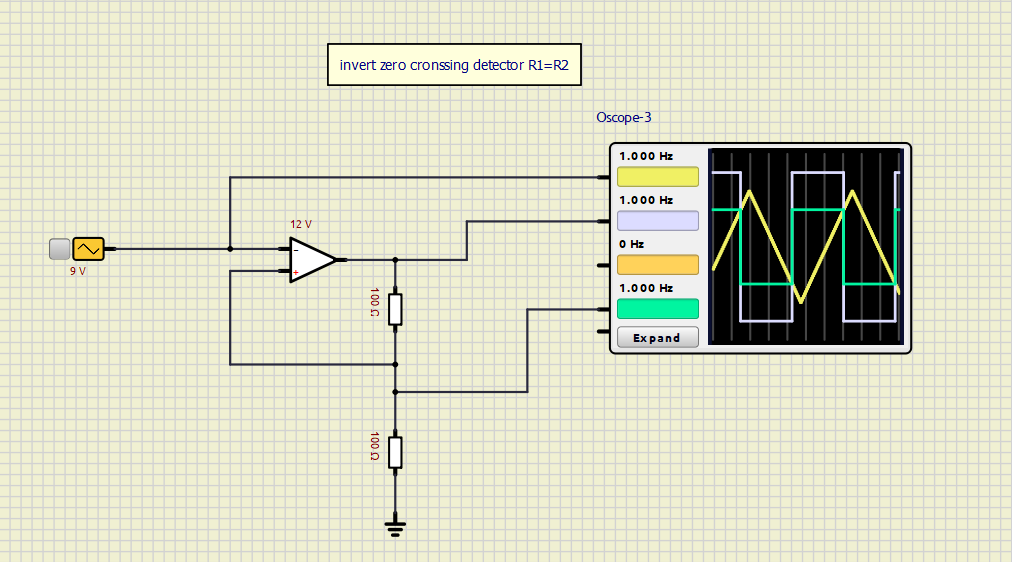
\includegraphics[width=8cm]{izcd r=r.png}
\end{center}

Sesuai perhitungan dengan rumus $V_{UT}^{+}$ dan $V_{LT}^{-}$:

\begin{equation}
    V_{UT}^{+}, V_{LT}^{-} = \pm 12 \cdot \frac{200}{300} \approx \pm 6 \text{ V}
\end{equation}


Sehingga didapatkan hasil $V_{UT}$ (gambar kiri) dan $V_{LT}$ (gambar kanan) sesuai simulasi adalah $\pm 6.120$ V yang dimana cukup sesuai dengan hasil teori yang didapat yakni $\approx 6$ V dan $V_{UT}$ adalah HIGH to LOW dan $V_{LT}$ adalah LOW to HIGH.

\begin{center}
    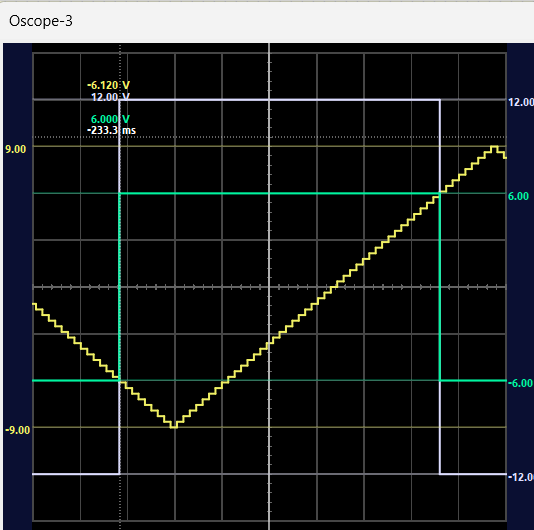
\includegraphics[width=8cm]{high1.png}
    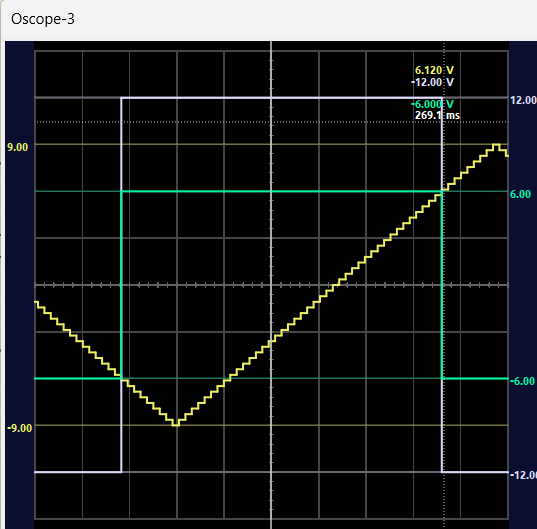
\includegraphics[width=8cm]{low1.png}
\end{center}


\section*{Heading lvl 3: Non-Inverting Zero Crossing with Hysterisis}
Non-inverting Zero Crossing Detector with Hysteresis adalah rangkaian op-amp yang mendeteksi perubahan sinyal terhadap nol dengan konfigurasi input di terminal non-inverting $(+)$ dan menggunakan hysteresis.

\begin{equation}
m = \frac{m_R}{R}
\end{equation}

\begin{equation}
V_{UT} = \frac{V_{sat}^{+}}{m}
\end{equation}

\begin{equation}
V_{LT} = \frac{V_{sat}^{-}}{m}
\end{equation}

Pada simulasi menggunakan $R = 100\Omega$ dan $m_R = 200\Omega$ sehingga $m = 2$. 
Kemudian menggunakan $V_{in} = \pm 9$ V dan $V_{cc}$ pada OpAmp $= \pm 12$ V, karena keadaan pada SimulIDE adalah ideal maka $V_{cc} = \pm V_{sat} = \pm 12$ V. Bentuk rangkaiannya seperti berikut ini:
\begin{center}
    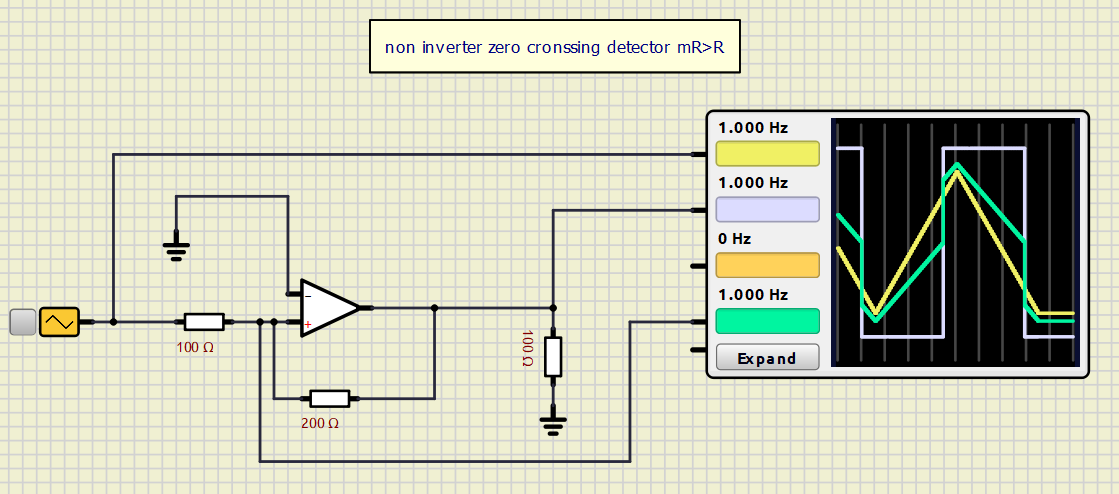
\includegraphics[width=10cm]{nizcd.png}
\end{center}
Dengan perhitungan menggunakan rumus $V_{UT}$ dan $V_{LT}$ pada NIZCD adalah:

\begin{equation}
V_{UT} = -\frac{V_{sat}^{+}}{m} = -\frac{12}{2} \approx -6 \text{ V}
\end{equation}

\begin{equation}
V_{LT} = -\frac{V_{sat}^{-}}{m} = -\frac{-12}{2} \approx +6 \text{ V}
\end{equation}


\begin{center}
    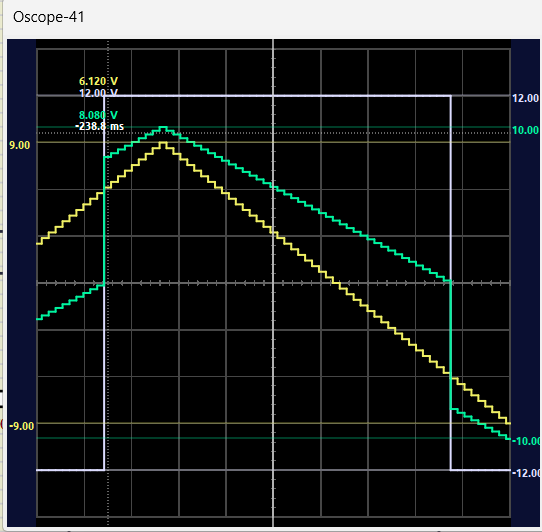
\includegraphics[width=8cm]{high2.png}
    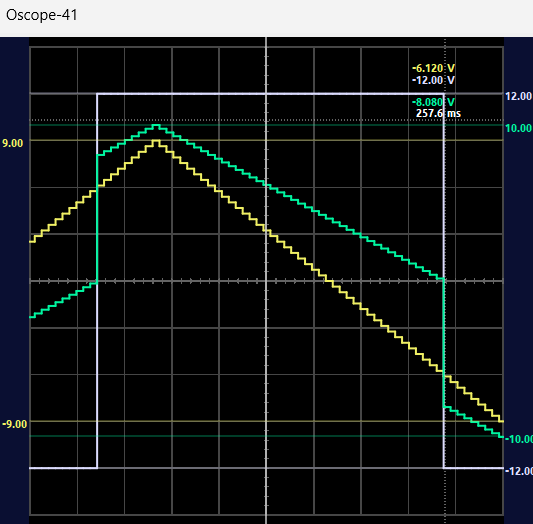
\includegraphics[width=8cm]{low2.png}
\end{center}

Gambar kiri adalah $V_{UT}$ dengan nilai $-6.120$ V dengan transisi dari \textit{low to high} dan gambar kanan adalah $V_{LT}$ dengan nilai $+6.120$ V dengan transisi dari \textit{high to low}. Nilai tersebut sesuai dengan hasil perhitungan $V_{UT}$ dan $V_{LT}$ yaitu sekitar $\pm 6$ V.





\end{document}
